\documentclass[../../main.tex]{subfiles}

% 

\begin{document}
\chapter{Základné charakteristiky spektrometrov}
Spektrometer je vedecké zariadenie, pôvodne používané na rozdelenie svetla do jednotlivo oddelených farieb, nazývaných spektrum. Spektrometer bol vyvinutý v raných štúdiách fyziky, astronómie a chémie. Spektrometre sa používajú v astronómii na analýzu chemického zloženia hviezd a planét. Koncepcia spektrometra teraz však zahŕňa aj nástroje, ktoré neskúmajú iba svetlo. Spektrometre môžu oddeľovať častice, atómy a molekuly na základe ich hmotnosti, hybnosti alebo energie. Tieto typy spektrometra sa používajú v chemickej analýze a fyzike častíc. Uveďme nejaké základné vlastnosti elektrónových spektrometrov: rozsah merania ($0.01-1000\,keV$), rozlíšenie ($10^{-8}-10^{-1}$), priestorový uhol do ktorého letia detekované elektróny ($0.0001-20 \% $ zo $4\pi$), transmisia T - časť z monoenergetického zväzku elektrónov ktoré prejdú do detektora, intenzita používaných magnetických polí $B=0.0001-3\,T$.


\section{Magnetický spektrometer}
V tomto druhu spektrometra sa magnetické pole využíva na určenie hybnosti (energie) elektrónu, poprípade inej častice. 
Behom doby boli využívané obzvlášť dva typy magnetických spektrometrov
\begin{itemize}
	\item \textbf{Rovinný spektrometer}\par
	Keď rýchlo nabitá častica (náboj $q$, hmotnosť $m$) vstúpi do konštantného magnetického poľa $B$, kde uhol medzi vektorom rýchlosti a magnetického poľa bude $90^{\circ}$, je v dôsledku Lorentzovej sily vychýlená do kruhovej dráhy o polomere r. Moment $p$ tejto častice je potom daný
	$$ p=mv=qBr, $$
	kde $m$ a $v$ sú hmotnosť a rýchlosť častice (viď obrázok \ref{js6:fig:rovinny_spektrometer}).\par
	\begin{figure}[!h]
	\centering
	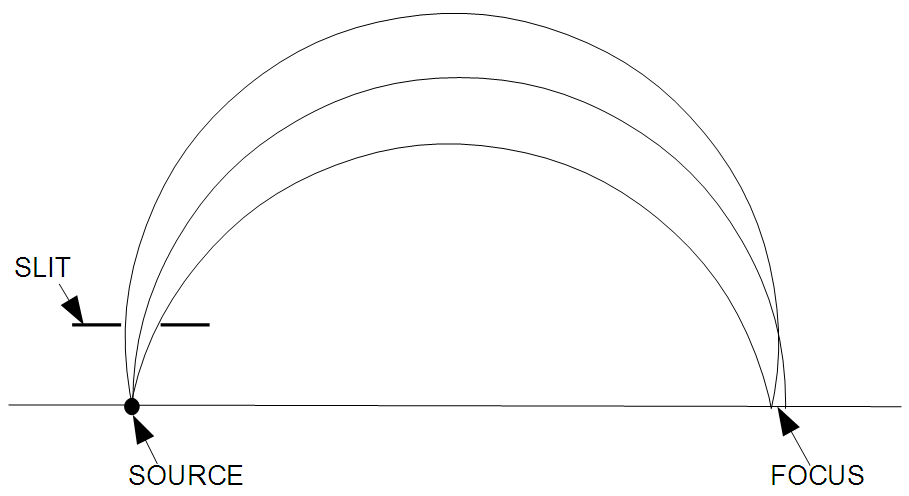
\includegraphics[width=0.5\textwidth]{js6-rovinny-spektrometer.png}
	\caption{Konštantné magnetické pole je kolmé na monitor/list papiera. Nabité častice o hybnosti $p$, ktoré prechádzajú štrbinou, sa odchyľujú do kruhových dráh s polomerom $r=p/qB$. Vidíme, že všetky častice narazili na vodorovnú čiaru na takmer rovnakom mieste. Tu by mal byť umiestnený čítač častíc.}
	\label{js6:fig:rovinny_spektrometer}
	\end{figure}
	\item \textbf{Šošovkový (čočkový) spektrometer}
	V tomto type spektrometra magnetické pole pôsobí ako magnetická šošovka (čočka) (viď obrázok \ref{js6:fig:sosovkovy_spektrometer}).
	\begin{figure}[!h]
	\centering
	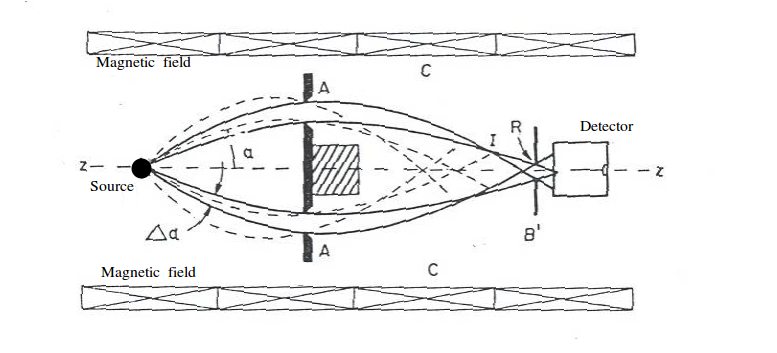
\includegraphics[width=0.9\textwidth]{js6-sosockovy-spektrometer.png}
	\caption{Princíp šošovkového spektrometra.}
	\label{js6:fig:sosovkovy_spektrometer}
	\end{figure} \newline
	Do tohto typu patri aj tzv. \textit{Orange} alebo \textit{Mini-orange} spektrometer. Tento spektrometer je magnetický, transportný a filtračný systém. Jedná sa o spektrometer, v ktorom magnetické pole usmerní elektróny emitované zdrojom k povrchu detektora (viď obrázok \ref{js6:fig:orange_spektrometer}). Názov tohto zariadenia je spôsobený súborom permanentných magnetov generujúcich pole. Tie sú tvarované ako pomarančové rezy a sú usporiadané v axiálnej symetrii.\par
	Permanentné magnety sú usporiadané symetricky okolo valcového absorbéra (napr. Pb-absorbér). Absorbér chráni detektor proti priamemu žiareniu zo zdroja.
	\begin{figure}[!h]
	\centering
	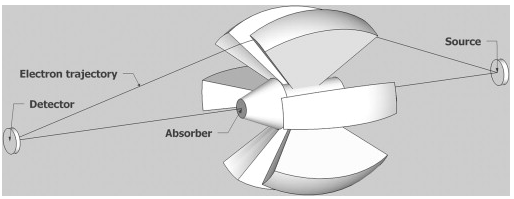
\includegraphics[width=0.7\textwidth]{js6-orange-spectrometer.png}
	\caption{Orange spektrometer: elektróny pochádzajúce zo zdroja sú fokusované na detektor cez toroidné magnetické pole generované súborom permanentných magnetov.}
	\label{js6:fig:orange_spektrometer}
	\end{figure}
	Zmenami zostavy magnetov sa dá meniť energia maxima transmisie (tým pádom aj účinnosť spektrometra).\par
	Niektoré spektrometre typu $Orange$ alebo $Mini-orange$ môžu byť využité ako transportéry. Úloha transportéru je nasledovná: majme prípad kedy meriame na zväzku. V tomto zväzku okrem častíc, ktoré chceme merať, máme aj vysoké pozadie fotónov alebo ďalších častíc. Magnetické pole transportérov je využité na transport elektrónov (alebo iných častíc) mimo toto pozadie. Energia elektrónu je následne určená kremíkovým detektorom. Využíva sa toroidné magnetické pole (pohyb po cykloide) alebo magnetické pole solenoidu (pohyb po špirále). Účinnosť systému je daná transmisiou transportného systému a účinnosťou detektora.
\end{itemize}
\textbf{Rozlíšenie magnetických spektrometrov}\par
Pohyb nabitej častice v magnetickom poli, v ktorom na nabitú časticu pôsobí sila $F_{M}=q\vec{v}\times \vec{B}$. V prípade, keď je vektor $\vec{B}$ kolmý na $\vec{v}$, môžme písať
$$ F=ma=m\frac{v^2}{r}=qvB $$ 
$$ mv=p=qBr $$
$$ R=\frac{\Delta p}{p}=\frac{\Delta(Br)}{Br} $$
kde používame relativistickú hmotnosť elektrónu $m=\frac{m_e}{\sqrt{1-(v/c)^2}}$. Takže $FWHM=\Delta(Br)$. Pre magnetické spektrometre mame rozlíšenie $R=10^{-3}-10^{-2}$.

\section{Elektrostatický spektrometer}
Používa sa pre energie častíc, ktoré nepresahujú $50$ keV. Pre vyššie energie častíc je potrebné príliš veľké napätie a je tu problém aj s relativistickou korekciou. V tomto spektrometre magnetické pole fokusuje elektróny do nejakého konkrétneho miesta, s využitím clon sa robí selekcia hybnosti (energie). Elektrické pole vytvára potenciálovú bariéru, ktorá prepustí elektróny s energiou vyššou ako je istý prah. Avšak namiesto bariéry sa môže robiť energetická selekcia častíc tak, že sa budú vyberať elektróny pomocou zakrivenia ich trajektórii v elektrickom potenciály  (viď obrázok \ref{js6:fig:elektrostaticky_spektrometer}).
\begin{figure}[!h]
\centering
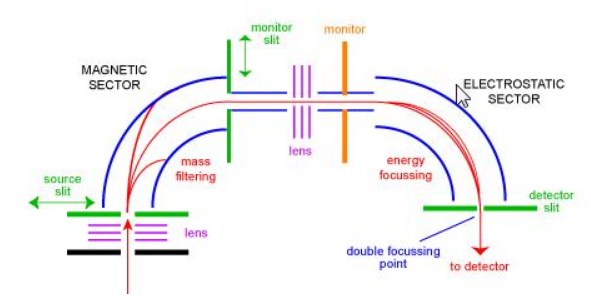
\includegraphics[width=0.9\textwidth]{js6-elektrostaicky-spektroskop.png}
\caption{Magneticky sektor vybera castice podla hmotnosti, to sme mali v predchadzajucom pripade. Avsak ako vidime elektrostaticky sektor sa zameriava na kineticke energie castic, kde castice s nevyhovujucou energiou narazia na steny. Namiesto tej zakrivenej casti mozme mat aj rovnu cast, kde bude nejaka potencialova bariera ktora nepusti castice, ktorych energia bude pod urcitym prahom potencialu.}
\label{js6:fig:elektrostaticky_spektrometer}
\end{figure}
S týmto elektrostatickým spektrometrom môžme spojiť napríklad tieto detektory:
\begin{itemize}
	\item \textbf{Kanálový násobič (channeltron)}\par 
	Je vhodny pre nizke energie ($\sim 1\,keV$). Channeltron je vyrobeny zo skla alebo keramiky. Povrch je z polovodicovej vrstvy. Zosilenie moze dosahovat hodnoty $\sim 10^7$. Funguje na principe sekundarnej emissie, kde jeden elektron indukuje emisiu dalsich elektronov (viď obrazok \ref{js6:fig:channeltron}). Mala citlivost na detekciu gama ziarenia.
	\begin{figure}[!h]
	\centering
	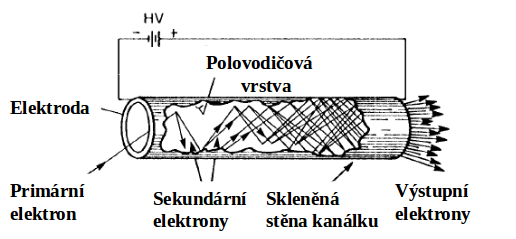
\includegraphics[width=0.9\textwidth]{js6-channeltron.png}
	\caption{Primarny elektron vyemituje niekolko elektronov. Tie nasledne pod vplyvom potencialu zrychlia a emituju dalsie elektrony. Tento proces bezi pokym zosilenie nie je dostatocne.}
	\label{js6:fig:channeltron}
	\end{figure} \newline
	Je tu moznost zoskupit viacej channeltronov do tkz. channeltron dosky - miliony miniaturnych zosilovacov pracuje nezavisle. Vdaka tejte dosticke vieme urcit polohu castice. Vzdialenost jednotlivych channeltronov v dosticke je zhruba $\sim 8-30\,\mu m$. Mala citlivost na magneticke pole a mrtva doba jednotlivych channeltronov je zhruba $\sim 10$ ns.
	\item \textbf{Kremíkové detektory}\par
	V tejto casti nebudeme velmi rozoberat kremikove detektory pretoze su podrobnejsie popisane v inej otazke. Vyhodou tychto detekorov je, ze mozu merat ako aj polohu tak aj energiu daneho elektronu. Pozname driftove komory, kde naboj z ionizacie driftuje k anode. Typicke driftove rychlosti su $\sim 5\,cm/\mu s$, z casu letu je mozne urcit polohu castice. Dalej pozname aj pixelove detekrory. Tento detektor sa sklada z jednotlivych pixelov, kde kazdy pixel ma vlastne vycitanie. Vieme urcit velmi presne polohu. 
\end{itemize}
Prikladom takehoto elektrostaickeho spektrometra je ESA12 – electrostatický spektrometer s vysokým rozlišením pro elektrony s energiemi $0-8$ keV, vhodný pro základní testy elektronových zdrojů vyvíjených pro projekt KATRIN - experiment zaoberajuci sa neutrinami.\newline
\textbf{Rozlíšenie elektrostatických spektrometrov}\par
Rozlisenie elektrostatickych spektrometrov je rozlisenim energie $R=\frac{\Delta E_{kin}}{E_{kin}}$, kde ${FWHM=\Delta E_{kin}}$. Da sa ukazat, ze vztah medzi magnetickym a elektrickym rozlisenim je nasledovny 
$$ \frac{dE_{kin}}{E_{kin}}=\bigg( 1+\frac{m_ec^2}{E_{kin}+m_ec^2}\bigg)\frac{d(Br)}{Br} $$ kde $$ \frac{dp}{p}=\frac{d(Br)}{Br}.$$
V nerelativistickej limite ($E_{kin} << m_ec^2$) mame $$ E_{kin}=\frac{p^2}{2m_e} \Rightarrow dE_{kin}=\frac{p}{m_e}dp $$
potom dostavame, ze $$ \frac{dE_{kin}/E_{kin}}{dp/p}=2.$$
Pre ultrarelativisticku limitu ($E_{kin} >> m_ec^2$) dostavame $$ E_{kin}=E=pc \Rightarrow \frac{dE_{kin}}{E_{kin}}=\frac{dp}{p} $$ potom dostavame $$ \frac{dE_{kin}/E_{kin}}{dp/p}=1.$$
Graficky vztah medzi energetickym a hybnostnym rozlisenim mame na obrazku \ref{js6:fig:rozslisenie}.
\begin{figure}[!h]
\centering
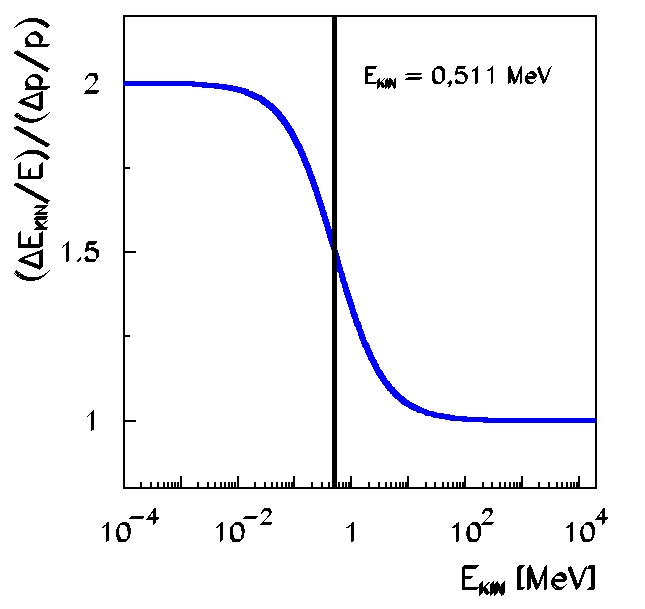
\includegraphics[width=0.5\textwidth]{js6-rozlisenie.png}
\caption{}
\label{js6:fig:rozslisenie}
\end{figure}

\section{Scintilačný spektrometer}
Zariadenie založené na scintilačnom čítači a používané na meranie takých vlastností jadrového žiarenia a elementárnych častíc ako intenzita žiarenia, energia častíc a životnosť nestabilných jadier a častíc.
Scintilatory casto konvertuju jediny vysoko-energeticky foton na velky pocet fotonov s nizsou energiou. Meranim intenzity zablesku (pocet fotonov vytvorenych r\"{o}ntgenovym alebo gamma fotonom) je mozne rozoznat povodnu energiu fotonu.\par
Spektrometer pozostáva z vhodného scintilátorového kryštálu, fotonásobovacej trubice (bacha fotonasobic a channeltron nie su to iste aj ked robia skoro to iste) a obvodu na meranie výšky impulzov produkovaných fotonásobičom. Impulzy sú spočítané a triedené podľa ich výšky, čím sa vytvorí x-y graf zábleskového scintilačného jasu v porovnaní s počtom zábleskov, ktoré sa približujú energetickému spektru dopadajúceho žiarenia s niektorými ďalšími artefaktmi. Monochromatické gama žiarenie produkuje fotopeak pri svojej energii (foton nestratil ani cast svojej energie). Avsak nie vzdy zachytime uplne celu energiu ziarenia. Detektor taktiez zachytava mensie energie gama ziarenia. Tieto straty boli sposobene Comptonovskym roptylom. Ďalej v spektre mozme pozorovat dva mensie píky, ktorych energia bude o $0.511\,MeV$ a $1.022\,MeV$ mensia ako pre povodny foton, ktore zodpovedajú tvorbe elektron-pozitronoveho paru, kde jeden alebo oba anihilacne fotony su zaznamenane, dalej este mozme vidiet tkz. beackscatter peak, ktory vznika, ked foton interaguje nie so scintilatorom ale so stenami detektora, pricom prostrednictvom Comptonovského rozptylu alebo fotoefektu vznika ziarenie, ktoreho energia je o dost menšia ako mal povodny foton.\par
Z dôvodu ich vysokej účinnosti pri zaznamenávaní rôznych častíc a žiarenia a ich rýchlej odozvy sa scintilačné spektrometre široko používajú v jadrovej spektroskopii a spektroskopii častíc s vysokou energiou. Pri nízkych energiách ($\leq1\,MeV$) je energetické rozlíšenie scintilačných spektrometrov nižšie ako pri proporčných počítadlách a polovodičových detektoroch. Krystaly, kore sa pouzivaju ako scintilacne materialy, mozu napriklad byt CsI v krystalickej forme (na detekciu protonov alebo alfa castic), ZnS (siroko sa vyuziva ao detektor alfa castic), NaI(Tl) (pouziva sa ako scintilator na detekciu gama ziarenia), LiI (na detekciu neutronov).\par
Vo vysoko-energetickej fyzike sa občas používajú veľké segmentové scintilačné spektrometre s úplnou absorpciou na meranie energie prichádzajúcej častice s $~10-100\,GeV$. Hmotnosť scintilátora v takýchto spektrometroch dosahuje desiatky alebo stovky ton. Meranie celkovej energie uvoľnenej v jadrovej kaskáde umožňuje určiť energiu prichádzajúcej častice s presnosťou až do $\pm10\%$.

\section{Polovodičový spektrometer}
Zariadenie na meranie rôznych charakteristík jadrového žiarenia a elementárnych častíc. Jeho hlavným prvkom je polovodičový detektor. Polovodičové spektrometre sa používajú napríklad na meranie spektra a  žiarenia a na izoláciu jadrových reakcií určitého druhu. Viackanálové analyzátory a elektronické počítače vo všeobecnosti tvoria koncovú časť polovodičového spektrometra. Na dosiahnutie vysokého rozlíšenia energie sa polovodičové spektrometre a predzosilňovače chladia umiestnením do kryostatu. Intenzivne sa vyuzivaju kremikove ale aj germaniove polovodicove detektory. Energeticke rozlisenie tychto detektorov sa pohybuje medzi hodnotamy $\sim 0,9-1,9\,keV$ pre castice s energiou $100-1000\,keV$. V zavislti od toho ake hodnoty energie chceme si volime material a hrubku okienka daneho detektora. Na obrazku \ref{js6:fig:BEGe}
mozme vidiet prierez germanioveho detektora, na ktorom vidime aj spominane okienko. Material a hrubka okienka sa meni kvoli absorpcii materialy. V tychto typoch sa vyuzivaju vyššie spominane magneticke transportery, ktore prepravuju elektrony do miesta s mensim pozadim. Vo väčších experimentoch ako napriklad LHC, sa vyuzivaju aj pozicne citlive detektory: kremikové stripove detektory (SSD), kremikové pixelove detektory (SPD) alebo kremikové driftove detektory (SDD).
\begin{figure}[!h]
\centering
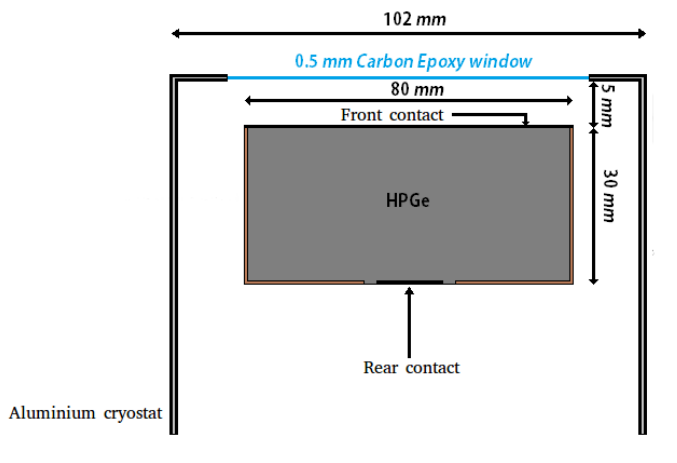
\includegraphics[width=0.4\textwidth]{js6-BEGe.png}
\caption{Prierez germaniového detektora typu BEGe. Vidime tiez spominane okienko. V tomto pripade je vyrobene z uhlika, co je dobre pre energie mensie ako $10\,keV$. Dalsie moznosti materialu pre toto okienko je napriklad hlinik, ktory je vhodny pre energie vacsie ako $30\,keV$ a pre energie mensie ako $3\,keV$ je najlepsie zvolit beryliove okienko.}
\label{js6:fig:BEGe}
\end{figure}\par

Na obrazku \ref{js6:fig:semiconductor_spectrometer} mozme vidiet priklad polovodicoveho spektrometra, ktory nesie nazov TATRA (TApe TRAnsportation) spektrometer. Bol navrhnuty a skonstruovany na Fyzikalnom ustave Slovenskej Akademie Vied. Tento system pozostava s vakuovej komory, troch koaxialnych HPGe detektorov (s $70-80\%$ efektivitou) a jedneho Broad Energy germanium detektora (BEGe), ktore merali gama ziarenie a jedneho Si(Li) detektora, ktory meral konverzne elektrony s energiou nad $100\,keV$ s rozlisenim $FWHM=1.3\,keV$. Vo vnutri komory je tlak $8\cdot 10^{-8}\,mbar$.

\begin{figure}[!h]
\centering
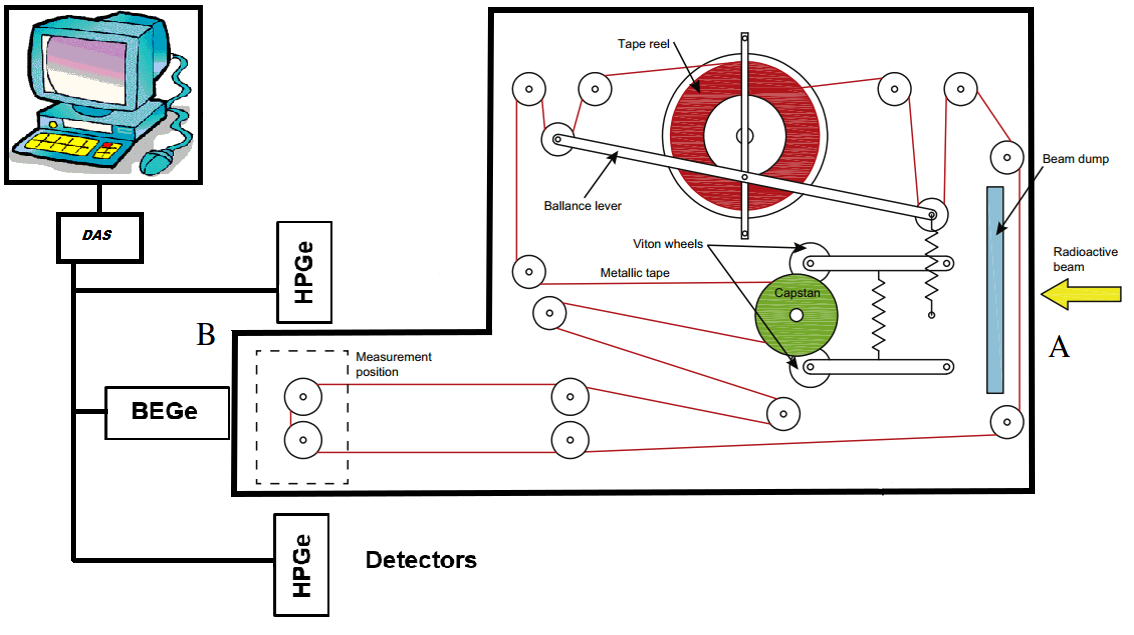
\includegraphics[width=0.8\textwidth]{js6-polovodicove-spektrometer.png}
\caption{Náčrt TATRA spektrometra. Podstatna cast je vo vnutri komory. Nasledne okolo toho vybezku su umiestnene detektory, ktore meraju to co je potrebne. Zmerane informacie su transportovane do Data Acquisision System. Tento spektroskop nevyuziva magneticke transportery ale funguje na paskovom principe, kde sa na jednom mieste naimplementuje vzorka na pasku (bod A) a posunie sa na miesto kde prebieha meranie (bod B).}
\label{js6:fig:semiconductor_spectrometer}
\end{figure}

\section{Kryštálový spektrometer}
Je to röntgenový spektrometer využívajúci kryštálovú mriežku. Tento spektrograf pozostáva z vysokonapäťového napájacieho zdroja ($50\,kV$ alebo $100\,kV$), širokopásmovej röntgenovej trubice zvyčajne s volframovou anódou a s berýliovym okienkom a držiakom na vzorku, analyzujúcim kryštálom, goniometrom a detektorom röntgenového žiarenia. Tieto komponenty sú usporiadané tak, ako je znázornené na obrázku \ref{js6:fig:crystal_spectrometer}. 
\begin{figure}[!h]
\centering
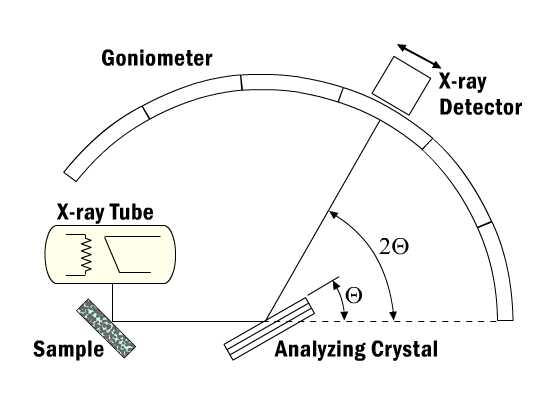
\includegraphics[width=0.5\textwidth]{js6-krystalovy-spektrometer.jpg}
\caption{Schéma kryštálového spektrometra.}
\label{js6:fig:crystal_spectrometer}
\end{figure}
Spojite r\"{o}ntgenové spektrum vychádzajúce z trubice ožaruje vzorku a excituje elektrony vo vzorke, ktore nasledne deexcituju a emituju charakteristicke ziarenie. Každý z 92 prvkov emituje jedinecne charakteristické spektrum. Na rozdiel od optického spektra je röntgenové spektrum pomerne jednoduché. Najsilnejšia čiara, zvyčajne z K-alpha prechodu, ale niekedy aj z L-alpha prechodu, postačuje na identifikáciu prvku. Existencia konkrétnej linky (ciary v spektre) preukazuje existenciu prvku a intenzita je úmerná množstvu konkrétneho prvku vo vzorke. Charakteristické ziarenie sa odráža od kryštálu (analyzátora) pod uhlom, ktorý je daný Braggovým zákonom $$ n\lambda = 2d\sin(\theta), $$ kde $\theta$ je difrakcny uhol, $n$ je stupen odrazu ($n=1,2,3...$) a $\lambda$ je vlnova dlzka ziarenie.\par 
Kryštál testuje všetky difrakčné uhly $\theta$ tak, ze sa pocas merania otáča. Detektor, ktory zachytava odrazene ziarenie sa taktiez otáča spolocne s krystalom. S citlivým detektorom sa röntgenové fotóny počítajú individuálne. Tieto hity sa môžu vykresliť v zavislosti od uhla odrazu. Charakteristické röntgenové lúče sa vyskytujú v špecifických uhloch a keďže je známa a zaznamenaná uhlová poloha pre každú rôntgenovú spektrálnu čiaru, je ľahké nájsť zloženie vzorky.


\end{document}